\documentclass[aspectratio=169,11pt]{beamer}

\usetheme{default}
\usecolortheme{default}
\setbeamertemplate{navigation symbols}{}
\setbeamertemplate{footline}{%
  \hfill\usebeamercolor[fg]{page number in head/foot}%
  \usebeamerfont{page number in head/foot}\insertframenumber\,/\,\inserttotalframenumber\hspace*{1em}\vspace*{0.6em}%
}
\setbeamercolor{structure}{fg=black!75}
\setbeamercolor{frametitle}{fg=black!85,bg=}
\setbeamercolor{title}{fg=black!85}
\setbeamercolor{block title}{fg=black!85,bg=black!6}
\setbeamercolor{block body}{bg=black!3}
\setbeamercolor{alerted text}{fg=black!80}
\setbeamercolor{local structure}{fg=black!70}
\setbeamertemplate{itemize item}{\textbullet}
\setbeamertemplate{itemize subitem}{--}
\setbeamertemplate{enumerate item}{\insertenumlabel.}
\setbeamerfont{frametitle}{series=\bfseries,size=\large}
\setbeamerfont{title}{series=\bfseries,size=\Large}

\usepackage{amsmath,amssymb}
\usepackage{booktabs}
\usepackage{graphicx}
\usepackage{siunitx}
\usepackage{multirow}
\usepackage{tikz}
\usetikzlibrary{arrows.meta,positioning,fit,backgrounds,calc}

\graphicspath{{../figures/}}

\title{Downscaling Municipal Soybean Yield Labels\\to Pixel Predictions with MSTNet}
\subtitle{Paran\'{a}, Brazil}
\author{Heitor Trielli Zanoni Ferreira}
\date{}

\begin{document}

\begin{frame}
  \titlepage
\end{frame}

\begin{frame}{Motivation}
  \begin{itemize}
    \item Yield estimates matter for food security, insurance, and risk.
    \item At scale, the best labels we have are municipal (IBGE PAM).
    \item Field-level evaluation needs finer maps $\Rightarrow$ downscaling.
    \item Gridded Sentinel-2, climate, and soil let us learn from coarse PAM and predict per soy pixel.
  \end{itemize}
  \vspace{0.7em}
  {\footnotesize Song et~al.\ (2022): PAM$\to$pixel with RF on phenology.
  We use multi-frequency Transformers and year leave-one-out.}
\end{frame}

\begin{frame}{Study area and data}
  \begin{itemize}
    \item Paran\'{a} soybean productivity from IBGE PAM (\si{t/ha}).
    \item MapBiomas soy mask (class 39) selects cells before aggregation.
    \item Sentinel-2: 10 L2A bands at $30\,\mathrm{m}\times 30\,\mathrm{m}$.
    \item Xavier climate: daily weather at $\sim 10\,\mathrm{km}\times 10\,\mathrm{km}$.
    \item MapBiomas Solo: clay, silt, sand, SOC at $30\,\mathrm{m}\times 30\,\mathrm{m}$ (0--30\,cm).
    \item Fixed season window: early October through late March.
    \item Keep municipality--years where MapBiomas soy area is $0.5$--$1.5\times$ PAM area.
  \end{itemize}
\end{frame}

\begin{frame}{Training path: municipal means}
  \centering
  \resizebox*{!}{0.82\textheight}{%
  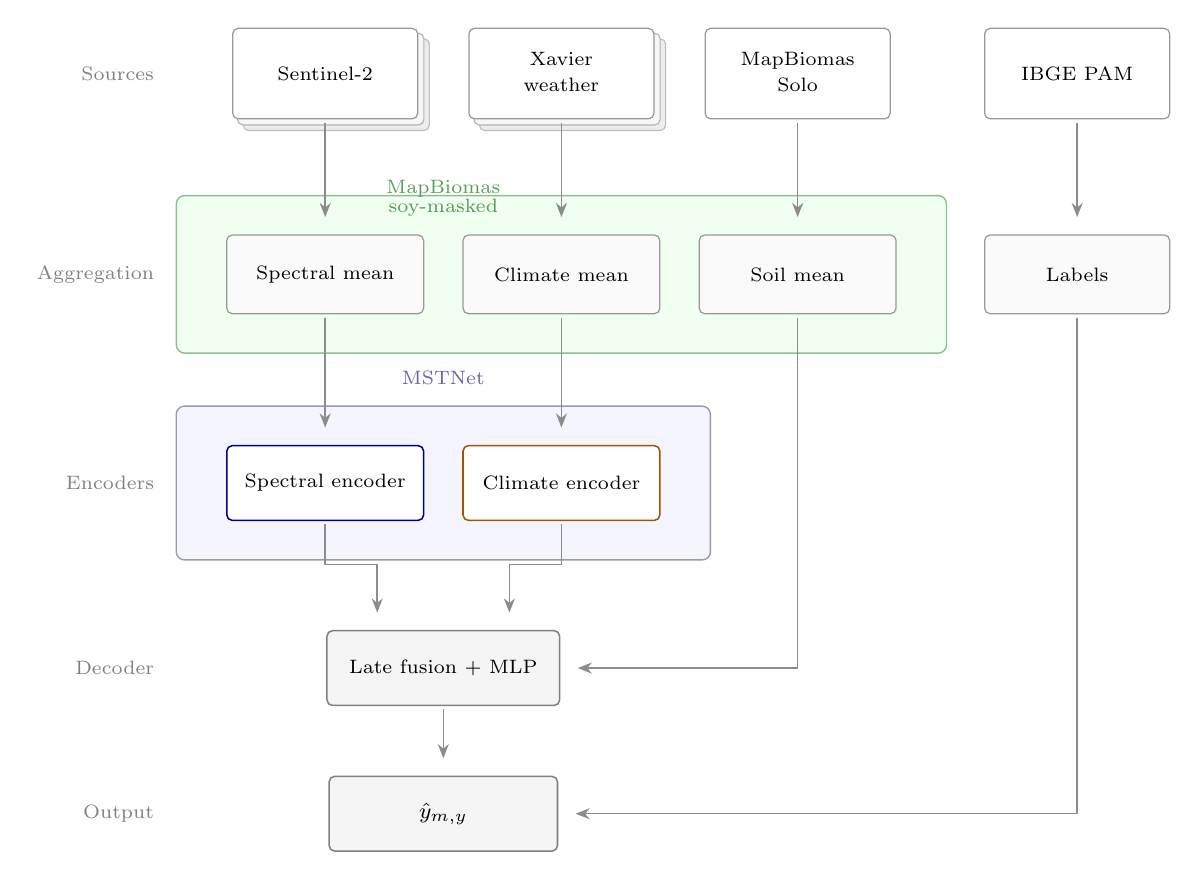
\begin{tikzpicture}[
    font=\footnotesize,
    line join=round,
    x=1cm, y=1cm,
    >={Stealth[length=1.8mm, width=1.4mm]},
    shorten >=2.2mm,
    shorten <=0.4mm,
    src/.style={
      draw=black!40, fill=white, rounded corners=2pt,
      align=center, inner xsep=5pt, inner ysep=5pt,
      minimum width=2.35cm, minimum height=1.15cm, line width=0.45pt
    },
    mid/.style={
      draw=black!40, fill=black!2, rounded corners=2pt,
      align=center, inner xsep=5pt, inner ysep=5pt,
      minimum width=2.35cm, minimum height=1.0cm, line width=0.45pt
    },
    encs/.style={
      draw=blue!55!black, fill=white, rounded corners=2pt,
      align=center, inner xsep=6pt, inner ysep=5pt,
      minimum width=2.5cm, minimum height=0.95cm, line width=0.55pt
    },
    encc/.style={
      draw=orange!65!black, fill=white, rounded corners=2pt,
      align=center, inner xsep=6pt, inner ysep=5pt,
      minimum width=2.5cm, minimum height=0.95cm, line width=0.55pt
    },
    dec/.style={
      draw=black!50, fill=black!4, rounded corners=2pt,
      align=center, inner xsep=8pt, inner ysep=6pt,
      minimum width=2.9cm, minimum height=0.95cm, line width=0.55pt
    },
    rowlab/.style={font=\scriptsize\color{black!50}, anchor=east},
    arr/.style={->, line width=0.55pt, draw=black!45},
  ]
    % Even 3.0cm columns; decoder at midpoint of spectral + climate
    \def\xs{-4.5}
    \def\xc{-1.5}
    \def\xso{1.5}
    \def\xlb{5.05}
    \def\xmid{-3.0}
    \def\xlab{-6.55}
    \def\yagg{-2.55}
    \def\yenc{-5.2}
    \def\ydec{-7.55}
    \def\yout{-9.4}
    \def\panelxsep{18pt}
    \def\panelasep{14pt}

    \node[rowlab] at (\xlab, 0) {Sources};

    \node[src] (s2) at (\xs, 0) {\scriptsize Sentinel-2};
    \begin{scope}[on background layer]
      \node[src, fill=black!7, draw=black!26, line width=0.4pt,
            inner sep=0pt, fit=(s2), xshift=4pt, yshift=-4pt] {};
      \node[src, fill=black!3, draw=black!30, line width=0.4pt,
            inner sep=0pt, fit=(s2), xshift=2pt, yshift=-2pt] {};
    \end{scope}

    \node[src] (xav) at (\xc, 0) {%
      \begin{tabular}{@{}c@{}}
        \scriptsize Xavier\\[0pt]
        \scriptsize weather
      \end{tabular}};
    \begin{scope}[on background layer]
      \node[src, fill=black!7, draw=black!26, line width=0.4pt,
            inner sep=0pt, fit=(xav), xshift=4pt, yshift=-4pt] {};
      \node[src, fill=black!3, draw=black!30, line width=0.4pt,
            inner sep=0pt, fit=(xav), xshift=2pt, yshift=-2pt] {};
    \end{scope}

    \node[src] (soil) at (\xso, 0) {%
      \begin{tabular}{@{}c@{}}
        \scriptsize MapBiomas\\[0pt]
        \scriptsize Solo
      \end{tabular}};
    \node[src] (pam) at (\xlb, 0) {\scriptsize IBGE PAM};

    \node[rowlab] at (\xlab, \yagg) {Aggregation};
    \node[mid, minimum width=2.5cm] (a_s2) at (\xs, \yagg) {\scriptsize Spectral mean};
    \node[mid, minimum width=2.5cm] (a_cl) at (\xc, \yagg) {\scriptsize Climate mean};
    \node[mid, minimum width=2.5cm] (a_so) at (\xso, \yagg) {\scriptsize Soil mean};
    \node[mid] (a_lb) at (\xlb, \yagg) {\scriptsize Labels};

    \begin{scope}[on background layer]
      \node[
        fit=(a_s2)(a_cl)(a_so),
        fill=green!6,
        draw=green!45!black!45,
        rounded corners=3pt,
        inner xsep=\panelxsep,
        inner ysep=\panelasep,
        line width=0.5pt
      ] (maskbox) {};
    \end{scope}
    \node[
      font=\scriptsize\color{green!40!black!65},
      align=center,
      anchor=south,
      inner sep=0pt
    ] at ([yshift=-8pt]\xmid,0 |- maskbox.north) {%
      MapBiomas\\[-1pt]
      soy-masked};

    \draw[arr] (s2.south) -- (a_s2.north);
    \draw[arr] (xav.south) -- (a_cl.north);
    \draw[arr] (soil.south) -- (a_so.north);
    \draw[arr] (pam.south) -- (a_lb.north);

    \node[rowlab] at (\xlab, \yenc) {Encoders};
    \node[encs] (e_s2) at (\xs, \yenc) {\scriptsize Spectral encoder};
    \node[encc] (e_cl) at (\xc, \yenc) {\scriptsize Climate encoder};

    \begin{scope}[on background layer]
      \node[
        fit=(e_s2)(e_cl),
        fill=blue!4,
        draw=blue!25!black!40,
        rounded corners=3pt,
        inner xsep=\panelxsep,
        inner ysep=\panelasep,
        line width=0.5pt
      ] (encbox) {};
    \end{scope}
    \node[font=\scriptsize\color{blue!40!black!60}, anchor=south]
      at ([yshift=4pt]encbox.north) {MSTNet};

    \draw[arr] (a_s2.south) -- (e_s2.north);
    \draw[arr] (a_cl.south) -- (e_cl.north);

    \node[rowlab] at (\xlab, \ydec) {Decoder};
    \node[dec] (dec) at (\xmid, \ydec) {\scriptsize Late fusion + MLP};

    \draw[arr] (e_s2.south) -- ++(0,-0.55) -| (dec.150);
    \draw[arr] (e_cl.south) -- ++(0,-0.55) -| (dec.30);
    \draw[arr] (a_so.south) -- (a_so.south |- dec.east) -- (dec.east);

    \node[rowlab] at (\xlab, \yout) {Output};
    \node[dec] (out) at (\xmid, \yout) {$\hat{y}_{m,y}$};

    \draw[arr] (dec.south) -- (out.north);
    \draw[arr] (a_lb.south) -- (a_lb.south |- out.east) -- (out.east);
  \end{tikzpicture}%
  }
\end{frame}

\begin{frame}{MSTNet architecture}
  \centering
  \includegraphics[width=\textwidth,height=0.85\textheight,keepaspectratio]{mstnet_arch.pdf}
\end{frame}

\begin{frame}{After training: pixel scoring}
  \begin{itemize}
    \item Training used municipal means; inference can use all soy pixels.
    \item Same weights $f_\theta$ score every soy pixel in a municipality.
    \item Inputs are the raw pixel values.
    \item Average pixel scores $\to$ municipal prediction (or any polygon).
    \item We could train pixel-wise, but it is too costly.
  \end{itemize}
\end{frame}

\begin{frame}{Evaluation}
  \begin{itemize}
    \item \textbf{Year LOO} (primary)
      \begin{itemize}
        \item Leave one harvest year out (2020--2024).
        \item Train on the other four; report only the held-out year.
        \item Select checkpoints on municipal-mean; also score the pixel path.
      \end{itemize}
    \item \textbf{Spatial holdout}
      \begin{itemize}
        \item Hold out 20\% of municipalities; seasons appear in both pools.
        \item Tests unseen places in known years.
      \end{itemize}
  \end{itemize}
\end{frame}

\begin{frame}{Year-LOO metrics}
  \centering
  \footnotesize
  \setlength{\tabcolsep}{4pt}
  \begin{tabular}{lcccccc}
    \toprule
    & & \multicolumn{2}{c}{Municipal-mean} & \multicolumn{2}{c}{Pixel path} & \\
    \cmidrule(lr){3-4} \cmidrule(lr){5-6}
    LOO year & $n$ & RMSE & $R^2$ & RMSE & $R^2$ & $\Delta R^2$ \\
    \midrule
    2020 & 346 & 0.411 & 0.233 & 0.395 & 0.291 & $+0.058$ \\
    2021 & 343 & 0.320 & \textbf{0.410} & 0.323 & \textbf{0.402} & $-0.008$ \\
    2022 & 342 & 1.342 & $-0.300$ & 1.404 & $-0.422$ & $-0.122$ \\
    2023 & 339 & 0.433 & 0.199 & 0.424 & 0.231 & $+0.032$ \\
    2024 & 336 & 0.577 & 0.259 & 0.568 & 0.284 & $+0.025$ \\
    \midrule
    Mean & --- & 0.617 & 0.160 & 0.623 & 0.157 & $-0.003$ \\
    Mean excl.\ 2022 & --- & 0.435 & 0.275 & 0.427 & \textbf{0.302} & $+0.027$ \\
    \bottomrule
  \end{tabular}

  \vspace{0.7em}
  {\footnotesize RMSE in \si{t/ha}.}
\end{frame}

\begin{frame}{Predicted vs.\ observed}
  \centering
  \includegraphics[width=\textwidth,height=0.78\textheight,keepaspectratio]{scatter_panel.pdf}
\end{frame}

\begin{frame}{Drought year 2022}
  \begin{columns}[T]
    \begin{column}{0.48\textwidth}
      \begin{itemize}
        \item Only drought year in the panel.
        \item Left out $\Rightarrow$ regime unseen in training.
        \item Over-predicts West / Northwest.
        \item OOD stress test, not a typical fold.
      \end{itemize}
    \end{column}
    \begin{column}{0.50\textwidth}
      \centering
      \includegraphics[width=\textwidth]{map_error_panel.png}
      {\scriptsize Best fold (2021) vs.\ drought fold (2022).}
    \end{column}
  \end{columns}
\end{frame}

\begin{frame}{Partial-season scoring}
  \centering
  \includegraphics[width=0.88\textwidth,height=0.62\textheight,keepaspectratio]{incomplete_series_r2.pdf}

  \vspace{0.3em}
  {\footnotesize Excl.\ 2022: mean $R^2$ reaches $0.288$ by February, $0.302$ with full Oct--Mar.}
\end{frame}

\begin{frame}{Intramunicipal maps (Mambor\'{e})}
  \centering
  \includegraphics[width=\textwidth,height=0.72\textheight,keepaspectratio]{mambore_panel.png}

  \vspace{0.2em}
  {\footnotesize Qualitative downscaling---no field yields to validate against.}
\end{frame}

\begin{frame}{Modality ablations (pixel path)}
  \centering
  \footnotesize
  \begin{tabular}{lcc}
    \toprule
    Variant & Mean $R^2$ & Excl.\ 2022 \\
    \midrule
    Full MSTNet (S2 + climate + soil) & 0.157 & \textbf{0.302} \\
    No soil & 0.147 & 0.234 \\
    No climate & $-0.112$ & $-0.017$ \\
    No Sentinel-2 & $-0.027$ & 0.040 \\
    \bottomrule
  \end{tabular}

  \vspace{0.9em}
  \begin{itemize}
    \item Ordinary years: climate $\gg$ Sentinel-2 $\gg$ soil.
  \end{itemize}
\end{frame}

\begin{frame}{Spatial holdout (80/20 municipalities)}
  \centering
  \footnotesize
  \begin{tabular}{lcccc}
    \toprule
    Subset & $n$ & RMSE & MAE & $R^2$ \\
    \midrule
    2020 & 70 & 0.330 & 0.262 & 0.426 \\
    2021 & 68 & 0.305 & 0.233 & 0.409 \\
    2022 & 69 & 0.694 & 0.468 & \textbf{0.636} \\
    2023 & 68 & 0.411 & 0.323 & 0.283 \\
    2024 & 68 & 0.385 & 0.300 & 0.581 \\
    \midrule
    Mean (intra-year) & --- & 0.425 & 0.317 & 0.467 \\
    Pooled & 343 & 0.448 & 0.317 & \textbf{0.736} \\
    \bottomrule
  \end{tabular}

  \vspace{0.7em}
  {\footnotesize RMSE/MAE in \si{t/ha}. Municipal-mean path; seasons appear in both pools.}
\end{frame}

\begin{frame}{Limits and next steps}
  \begin{itemize}
    \item The model often gets the year right but ranks municipalities poorly within a year.
    \item Management, cultivar, and planting cycle are unobserved.
    \item Next: ranking / correlation losses, stress-aware climate pooling, more drought years in training.
  \end{itemize}
\end{frame}

\begin{frame}
  \centering
  \vspace{2.5cm}
  {\Large Thank you}
\end{frame}

\end{document}
